\section{FURTHER OPTIMIZATION BY V\textsubscript{TH} ASSIGNMENT}
\label{sec:TVA}
% (1)
In the section, V\textsubscript{th} assignment and aging manipulation are applied together to further optimize the required $T_c$. In addition to aging manipulation based on DCC insertion/deployment, we re-assign the threshold voltage of certain clock buffers, such that the latencies of the buffers are changed, so are the slacks, which give us the opportunity to further mitigate the aging-induced degradation of logic network based on timing borrowing. The section is organized as follows:~\ref{sec:TVA:example} demonstrates how V\textsubscript{th} assignment further optimizes the required $T_c$.~\ref{sec:TVA:leader} introduces the rule/mechanism of V\textsubscript{th} assignment, followed by~\ref{sec:TVA:leaderconstraint}, which explains how we convert the rule/mechanism into CNF clauses.~\ref{sec:TVA:timingconstraint} introduces the new timing constraints when V\textsubscript{th} assignment is considered. Finally,~\ref{sec:TVA:experiment} shows the experimental results, which is optimized based on DCC insertion and V\textsubscript{th} assignment.

% (2)
\subsection{Motivating Example considering V\textsubscript{th} assignment}
\label{sec:TVA:example}
We use the illustrative example to explain how we further improve the aging tolerance by comparing the two examples of Section~\ref{sec:motivate} and this section, based on the design in Figure~\ref{fig:sub:example}. The example in Section~\ref{sec:motivate} only considers the aging manipulation based on DCC deployment/insertion; however, in this section, the two approaches, DCC deployment and V\textsubscript{th} assignment are applied together to optimize/reduce required $T_c$. We let the DCC deployment same with that in the first example (in Section~\ref{sec:motivate}), i.e., 20\% DCC and 80\% DCC are inserted at the inputs of buffer 1 and buffer 2, respectively. Moreover, we begin re-assigning high V\textsubscript{th} to the certain clock buffers, which are in the intervals from buffer 2 to \ce{FF_x} and  to \ce{FF_y}. In other words, buffer 2 and its downstream buffers are re-assigned to high V\textsubscript{th}. To include the aging rates of HTV (High Threshold Voltage, or High-V\textsubscript{th}) buffers in the setup-time constraint, we assume that, the fresh/non-aging delay of HTV buffer is 1.2X longer than that of nominal buffer (whose V\textsubscript{th} are not reassigned), and aging rates of HTV buffer, with the duty cycle of 20\%, 40\%, 50\% and 80\%, are 0.5\%, 4.1\%, 5.4\% and 8.2\%, respectively. Note that, the aging rates of HTV buffer are lower than those of nominal buffer, because the higher/lower V\textsubscript{th} leads to lower/higher aging rates~\cite{chen2013novel}. Consider the new aging factors in the setup-time constraints on \ce{L_{XY}} and \ce{L_{YZ}}:
\begin{equation}
	\mbox{\fontsize{8}{9.6}\selectfont \ce{L_{XY}}:\quad$\textbf{1.09}C_X+1.2T_{cq}+1.15D_{XY}+1.2T_{su}<\textbf{(1.2+0.08)}C_Y+T_c$} 
	\label{eq:lxy2}
\end{equation}
\begin{equation}
	\centering
	\mbox{\fontsize{8}{9.6}\selectfont \ce{L_{YZ}}:\quad$\textbf{(1.2+0.08)}C_Y+1.2T_{cq}+1.15D_{YZ}+1.2T_{su}<\textbf{(1.2+0.08)}C_Z+T_c$} 
	\label{eq:lyz2}
\end{equation}
By re-arranging Equations (\ref{eq:lxy2}) and (\ref{eq:lyz2}):
\begin{flalign*}
	\hspace{1.2em}\ce{L_{XY}}: T_c &> 96.5 &\\
	\hspace{1.2em}\ce{L_{YZ}}: T_c &> 104
\end{flalign*}

Apparently, the required $T_c$ is further reduced/optimized from 108.5 (in Section~\ref{sec:motivate}) to 104 by inserting two DCCs and V\textsubscript{th} assignment in the existing synthesized clock network. We also observe that, the required $T_c$ is not dominated by \ce{L_{XY}} anymore (in Section~\ref{sec:motivate}); instead, it turns out that \ce{L_{YZ}} dominates $T_c$. As it can be seen, when the two approaches, V\textsubscript{th} assignment and aging manipulation  (by DCC insertion), are applied together, the skew for \ce{L_{XY}}, which equals 1.28$C_Y$ minus 1.09$C_X$, is larger than that in Section~\ref{sec:motivate}. Therefore, the new skew for \ce{L_{XY}} is more useful/beneficial and accounts for the better optimization of required $T_c$. 
Additionally, when it comes to the timing-borrowing mechanism of the two examples, there exists a difference: The timing-borrowing mechanism in Section~\ref{sec:motivate}, is achieved by the aging-induced clock skew, caused by manipulating the duty-cycle delivered to flip-flops. However, in the example, the timing-borrowing mechanism is based on aging-induced clock skew and \textit{tech-induced} clock skew, which is caused by manipulating the technology of clock buffers, i.e., re-assign the V\textsubscript{th} of clock buffers. 

% (3)
\subsection{Technology Leader}
\label{sec:TVA:leader}
When V\textsubscript{th} assignment is considered, how to select shortlisted clock buffers arises as a problem. The so-called shortlisted buffers are those whose V\textsubscript{th} will be re-assigned (i.e., their technology is changed). Because the count and the combination of shortlisted buffers are numerous, we need to reduce the complexity of the problem. Thus, we introduce the rule of V\textsubscript{th} assignment by explaining \textit{technology leader}. 

If the clock buffer is chosen as the \textit{technology leader}, the clock buffer and its downstream buffers are regarded as shortlisted buffers. In other words, the technology of the buffer and the downstream buffers will be replaced with new counterpart. For example, in~\ref{sec:TVA:example}, buffer 2 is actually chosen as the technology leader, so that the shortlisted buffers are buffer 2 and its downstream buffers, which also include buffer 3. Note that, there is a difference between DCC and technology leader. DCC is not a clock buffer but a special-purpose gate, which is inserted at the input of the clock buffer to manipulate the aging rates of downstream buffers; however, technology leader is an existing clock buffer. More specifically, it is selected from the buffers in the clock tree and indicates where we begin manipulating the technology of downstream buffers toward flip-flops.

% (4)
\subsection{Proposed Framework considering V\textsubscript{th} Assignment}
\label{sec:TVA:framework}
\begin{figure}
	\centering
	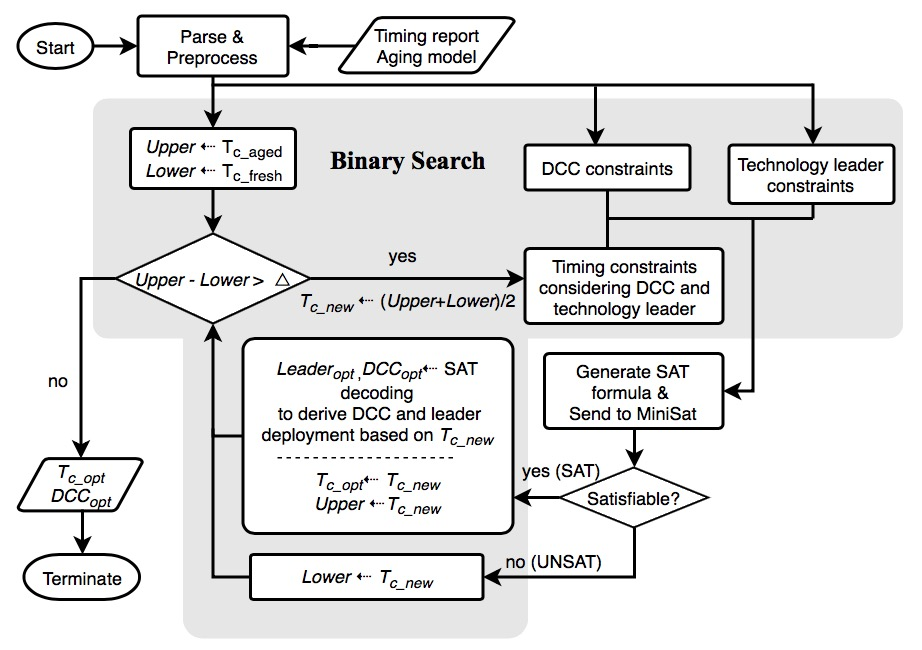
\includegraphics[width=0.9\columnwidth]{Flow_chart_tva.png}
	\caption{The overall flow of the framework when technology leaders are considered }
	\label{fig:flow:tva}
\end{figure}
The proposed framework, which considers aging manipulation (DCC) and V\textsubscript{th} assignment (technology leader), is depicted in Figure~\ref{fig:flow:tva}. Compared with the leader-free framework in Figure~\ref{fig:flow}, it is also based on a binary search for the minimum clock period ($T_c$) and SAT formulation. The problem of how to select technology leader is formulated as SAT problem, so is the problem of DCC insertion/deployment. In the sequel, Section~\ref{sec:TVA:leader_encode} explains how the problem of DCC insertion and technology leader selection is encoded by Boolean variables. Section~\ref{sec:TVA:leaderconstraint} introduces technology leader constraints, which is similar to DCC constraint. Section~\ref{sec:TVA:leaderconstraint} introduces the timing constraints which consider DCC deployment and technology leader selection. Finally,  Section~\ref{sec:TVA:leaderconstraint} shows the further optimized experimental results, based on DCC deployment and technology leader selection.

% (5)
\subsection{Encoding for DCC and Technology Leader Deployment}
\label{sec:TVA:leader_encode}
The problem of DCC deployment and technology leader selection needs to be encoded into Boolean representation before being transformed into a SAT-based formulation. Assume that a total of $N$ types of DCCs can be chosen. Including the DCC-free case where no DCC is inserted, there are ($N$ + 1) possibilities of DCC insertion for each clock buffer. Furthermore, we also assume that a total of $M$ types of technology leaders can be chosen. Note that, each technology represents an individual technology. Including the nominal technology, there are ($M$ + 1) possibilities of technology leader selection for each clock buffer. We denote a clock buffer by $p\left(1 \leq p \leq P\right)$ where $P$ is the number of buffers. For each buffer, Boolean variables $B_{p,q}\left(1 \leq p \leq P, 1 \leq q \leq Q = \lceil \lg (N + 1)(M + 1)\rceil \right)$ are introduced where $\left\{B_{p,1}, B_{p,2},\dotsc, B_{p,Q}\right\}$ encode the aforementioned ($N$ + 1)($M$ + 1) possibilities of DCC insertion at the input of buffer $p$.

Without loss of generality, we assume $N$ = 3, and $M$ = 1. Thus, there are 3 types of DCCs, which are assumed to be 20\%, 40\%, and 80\% DCCs, as shown in Figure~\ref{fig:dcctype}. In addition, there is 1 type of technology leader, which is assumed to be a HTV leader. Therefore, three Boolean variables are used for encoding eight possibilities of DCC and technology leader insertion at the input of any buffer. The eight possibilities can be encoded as follows:\newline

\begin{tabular}{ | c | c | c | c | }
	\hline
  	 & Leader type & DCC type & $\{B_{p,3}, B_{p,2}, B_{p,1}\}$ \\ \hline
  	(1)\quad & Nominal V\textsubscript{th} & None & \{0, 0, 0\} \\ \hline
  	(2)\quad & Nominal V\textsubscript{th} &20\% &  \{0, 0, 1\} \\ \hline
  	(3)\quad & Nominal V\textsubscript{th} &40\% &  \{0, 1, 0\} \\ \hline
  	(4)\quad & Nominal V\textsubscript{th} &80\% &  \{0, 1, 1\} \\ \hline
	(5)\quad & HTV & None & \{1, 0, 0\} \\ \hline
  	(6)\quad & HTV & 20\% &  \{1, 0, 1\} \\ \hline
  	(7)\quad & HTV & 40\% &  \{1, 1, 0\} \\ \hline
  	(8)\quad & HTV & 80\% &  \{1, 1, 1\} \\ \hline 
\end{tabular}

% (6)
\subsection{Technology Leader Constraint}
\label{sec:TVA:leaderconstraint}

% (7)
\subsection{Timing Constraint considering DCC and Technology Leader}
\label{sec:TVA:timingconstraint}

% (8)
\subsection{Experimental Results}
\label{sec:TVA:experiment}